\documentclass[brazil,14]{beamer}
\usepackage[utf8]{inputenc}
\usepackage{beamerthemesplit}
\usepackage{color}
\usepackage{xcolor}
\usepackage{amssymb}
\usepackage{amsmath}
\usepackage{fancybox}
\usepackage{ulem}
\usepackage{listingsutf8}
\usetheme{Copenhagen}
\usefonttheme{serif}
%\usetheme{CambridgeUS}
%\usetheme{Malmoe}
\setbeamertemplate{footline}[frame number]
\newenvironment{itemizespc}{
\begin{itemize}
  \setlength{\itemsep}{15pt}
}{\end{itemize}}

\xdefinecolor{darkblue}{rgb}{0,0,0.5}

\newcommand{\lyxline}[1][1pt]{%
  \par\noindent%
  \rule[.5ex]{\linewidth}{#1}\par}
  
  % -inicio codigo fonte\usepackage{listings}
\lstset{
  language=C,
  basicstyle=\ttfamily\scriptsize, 
  %basicstyle=\ttfamily\tiny,
  extendedchars=true, 
  showspaces=false, 
  showstringspaces=false, 
  numbers=left,
  numberstyle=\tiny,
  breaklines=true, 
  backgroundcolor=\color{yellow!8},
  breakautoindent=true, 
  captionpos=b,
  xleftmargin=0pt,
}
%\renewcommand{\lstlistlistingname}{Lista de Listagens}
% - fim codigo fonte

%\usebackgroundtemplate%
%{%
%    \includegraphics[width=\paperwidth,height=\paperheight]{maratona.png}%
%}

\begin{document}

\title{KnEDLe - Ferramentas de anotação}

%\begin{figure}
%\includegraphics[scale=0.3]{logoICMC.png}
%\end{figure}

%\author{May 15, 2015}




%\frame{\titlepage}

%-------------------------------------



%\frame{\frametitle{Corner point detection}
%\begin{itemizespc}
%\item Case 1
%\begin{figure}
%\includegraphics[scale=0.35]{figs/teste2.png}
%\end{figure}
%\end{itemizespc}
%}

%\frame{\frametitle{Corner point detection}
%\begin{itemizespc}
%\item Case 2
%\begin{figure}
%\includegraphics[scale=0.35]{figs/teste3.png}
%\end{figure}
%\end{itemizespc}
%}

\begin{frame}[plain]{}
\begin{center}
 Universidade de Brasília (UnB)\\
 Departamento de Ciência da Computação\\
 %{\bf }\\
\setbeamercolor{block body}{fg = white, bg=darkblue}
\vspace{0.75cm}
\begin{block}{ }
\begin{center}
\vspace{0.15cm}
\Large{ {\bf Estratégias para Anotação}}\\
\Large{ {\bf de Textos do DODF}}\\
\vspace{0.15cm}
\end{center}
\end{block}
\vspace{0.4cm}
{\bf Equipe KnEDLe/Data Annotation}\\
\vspace{0.4cm}
\vspace{0.25cm}

\includegraphics[width=0.2\linewidth]{figs/unb.png} \hspace{1cm}

\includegraphics[width=0.2\linewidth]{figs/logo_fapdf.png} \hspace{1cm}

\includegraphics[width=0.2\linewidth]{figs/logo_finatec.png}
\end{center}
\end{frame}


\frame{\frametitle{Equipe}
\begin{table}
\centering
\begin{tabular}{cc}
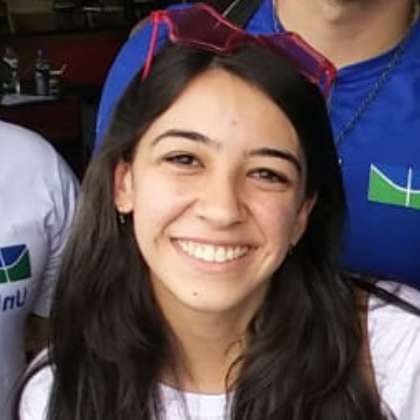
\includegraphics[width=0.3\linewidth]{figs/livia.png} \hspace{1cm} & 

\includegraphics[width=0.3\linewidth]{figs/matheus.jpg} \hspace{1cm} \\
Lívia & Matheus \\
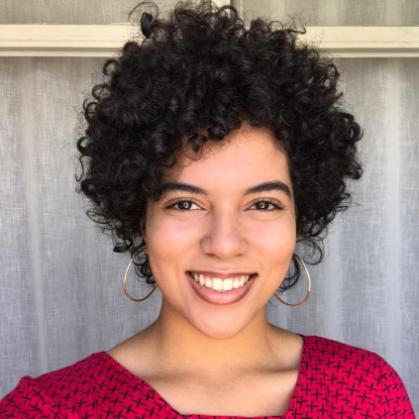
\includegraphics[width=0.3\linewidth]{figs/tatiana.jpg} \hspace{1cm} & 
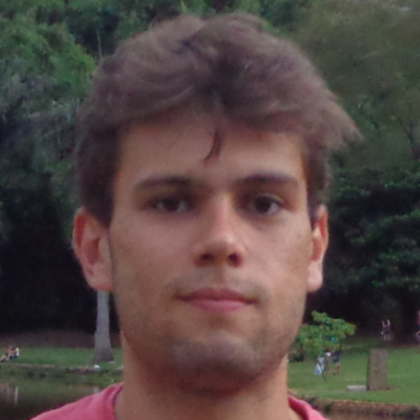
\includegraphics[width=0.3\linewidth]{figs/vinicius.png} \hspace{1cm} \\
Tatiana & Vinícius \\
\end{tabular}
\end{table}
}


%\frame{\frametitle{}
%\begin{center}
%\textbf{\Huge{Atividades}}\\
%\end{center}
%\begin{center}
%\includegraphics[width=0.3\linewidth]{figs/maratona.png}
%\end{center}
%}

\frame{\frametitle{Cenário}
\begin{itemizespc}
\item Algumas tarefas definidas no projeto KnEDLe se baseiam em abordagens supervisionadas de aprendizado de máquina (AM)
\begin{itemize}
\item classificação de textos
\item reconhecimento de entidades nomeadas
\end{itemize}
\item O aprendizado dos modelos de AM supervisionados depende de dados rotulados
\begin{itemize}
\item Os textos do Diário Oficial do Distrito Federal (DODF) são coletados sem informações de rótulos.
\end{itemize}
\end{itemizespc}
}

\frame{\frametitle{Aprendizado ativo}
\begin{itemizespc}
%\item O aprendizado ativo \footnote{Settles, B.. From theories to queries: Active learning in practice. Active Learning and Experimental Design (Workshop in conjunction with AISTATS, p. 1-18, 2011.} é um algoritmo iterativo que seleciona instâncias relevantes em um conjunto de dados para serem manualmente anotadas por um especialista;
%\item é uma eficiente abordagem que mantém a acurácia enquanto reduz o tamanho do conjunto de treinamento em várias tarefas de aprendizado de máquina.
\item \textbf{Princípio:} deve-se manter a acurácia de um modelo de AM treinado com menos dados rotulados quando comparado com o treinamento com todos os dados \footnote{\url{http://github.com/oraclesknedle/activeLearning_DODF}}
\begin{center}
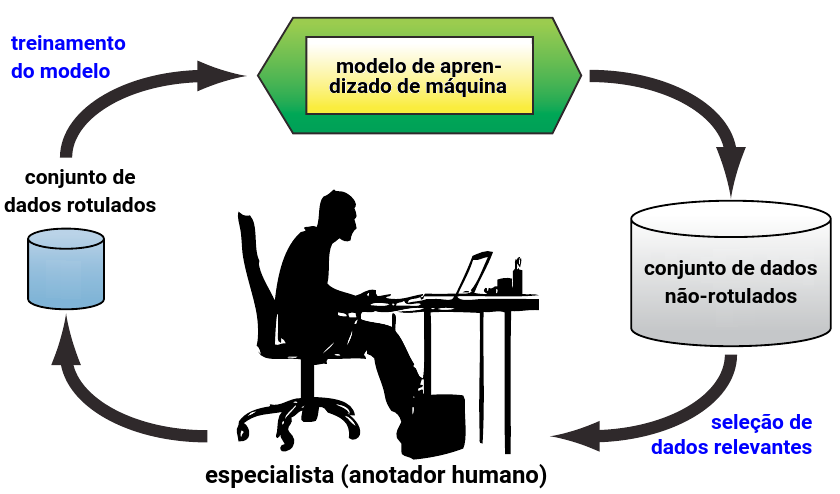
\includegraphics[width=0.8\linewidth]{figs/poolbased.png}
\end{center}
\end{itemizespc}
}

\frame{\frametitle{Representações de textos}
\begin{itemizespc}
\item Os textos do DODF são naturalmente não-estruturados;
\item Deve-se explorar representações estruturadas apropriadas;
\item Estudos \footnote{\url{http://github.com/oraclesknedle/text_experiments}} de representações para anotação de textos em modelos de classificação:
\begin{itemize}
\item Modelo espaço vetorial (\textit{Term Frequency-Inverse Document Frequency});
\item \textit{Word embeddings} (\textit{word2vec}, \textit{fastText}, \text{BERT}).
\end{itemize}
\end{itemizespc}
}

\frame{\frametitle{Mineração visual de textos}
\begin{itemizespc}
\item Visualização de coleções de textos para apoiar as tarefas de aprendizado de máquina e processamento de linguagem natural;
\item Empregar visualização interativa para gerar representações gráficas intuitivas dos textos, visando facilitar a interpretação dos padrões e relações de similaridade; 
\begin{center}
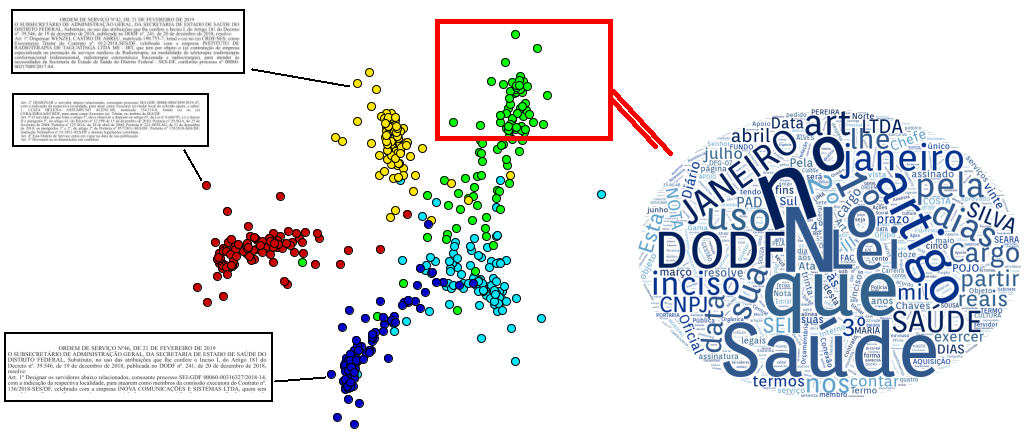
\includegraphics[width=0.8\linewidth]{figs/lsp.png}
\end{center}
\end{itemizespc}
}

\frame{\frametitle{Mineração visual de textos}
\begin{itemizespc}
\item Visualização de coleções de textos para apoiar as tarefas de aprendizado de máquina e processamento de linguagem natural;
\item Empregar visualização interativa para gerar representações gráficas intuitivas dos textos, visando facilitar a interpretação dos padrões e relações de similaridade; 
\item Integração de visualização com modelagem de tópicos para auxiliar os especialistas na anotação dos textos \footnote{\url{http://github.com/oraclesknedle/LDATopicModel}} e outras processos de descoberta de conhecimento.
%\begin{center}
%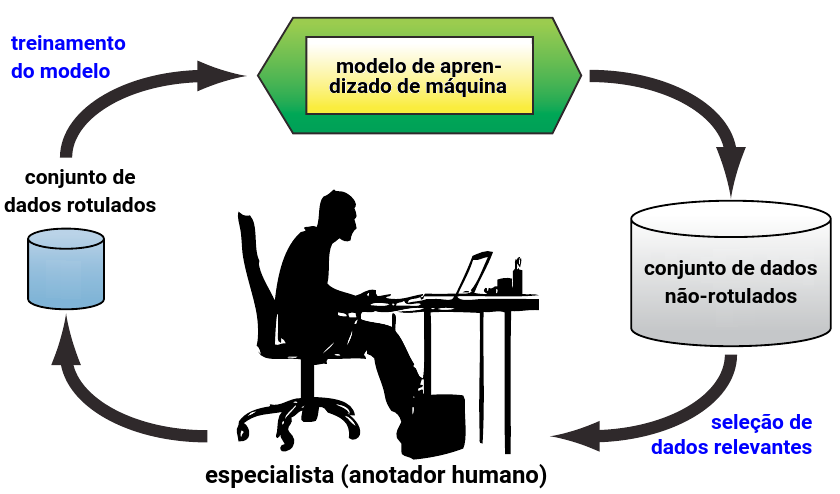
\includegraphics[width=0.8\linewidth]{figs/poolbased.png}
%\end{center}
\end{itemizespc}
}


%\frame{\frametitle{Cenário}
%\begin{itemizespc}
%\item Uso de outras coleções de textos:
%\begin{itemize}
%\item Diário Oficial da Prefeitura do Recife;
%\item Artigos científicos;
%\end{itemize}
%\item \textbf{Demanda:} geração de coleções de textos rotulados do DODF \textbf{padrão ouro} (\textit{gold standard})
%\end{itemizespc}
%}


\frame{\frametitle{Anotação de documentos}
\begin{itemizespc}
\item \textbf{Demanda:} geração de coleções de textos rotulados do DODF \textbf{padrão ouro} (\textit{gold standard});
\item A literatura relata que a anotação manual dos textos é a abordagem mais indicada \footnote{Wissler, L., Almashraee, M., Díaz, D. M., Paschke, A.. The Gold Standard in Corpus Annotation. In IEEE Germany Student Conference, 2014};
\begin{itemize}
\item A alta qualidade de \textit{Corpora} Gold Standard exige a análise das anotações por vários especialistas, de maneira independente;
\item Exige um grau de concordância para assegurar qualidade, tornando o processo extremamente custoso.
\end{itemize}
%\item Corpora com rótulos de alta qualidade e confiança são importantes, pois os erros nas categorias das instâncias são propagados no treinamento e no modelo de classificação final;
\item Anotação manual realizada pela ferramenta TeamTat \footnote{Islamaj, R., Kwon, D., Kim, S., Lu, Z.. TeamTat: a collaborative text annotation tool. arXiv preprint arXiv:2004.11894, 2020}
%#\begin{itemize}
%item URL: \url{https://www.teamtat.org/}
%\end{itemize}
\end{itemizespc}
}

\frame{\frametitle{}
\begin{center}
\textbf{\Huge{TeamTat}}\\
\end{center}
%\begin{center}
%\includegraphics[width=0.3\linewidth]{figs/maratona.png}
%\end{center}
}

%\frame{\frametitle{Limitações}
%\begin{itemizespc}
%\item Padrão heterogêneo dos blocos de textos do DODF em relação aos atos definidos no documento de requisitos;
%\begin{itemize}
%\item Ato de reversão com padrão confuso
%\end{itemize}
%\item Atos tornados sem efeito: quais atos relacionados à nomeação, exoneração e aposentadoria, são os mais relevantes?
%\end{itemizespc}
%}


%\frame{\frametitle{Colors}

%\textcolor{red}{Of course that you could color your text}
%\textcolor{orange}{Of course that you could color your text}
%\textcolor{blue}{Of course that you could color your text}
%\textcolor{yellow}{Of course that you could color your text}
%\textcolor{green}{Of course that you could color your text}

%}
%-------------------------------------

%\frame{\frametitle{Formating}

%\begin{center}
%\sout{strikethrough}  \\
%\textit{italic} \\
%\textbf{bold} \\
%\underline{underline}

%\end{center}

%}

\end{document}
